% Copyright (C)  2015  Alexander Jankowski, Philipp Hacker.
% Permission is granted to copy, distribute and/or modify this document
% under the terms of the GNU Free Documentation License, Version 1.3
% or any later version published by the Free Software Foundation;
% with no Invariant Sections, no Front-Cover Texts, and no Back-Cover Texts.
% The lincense itself can be found at <https://www.gnu.org/licenses/fdl-1.3>.

\documentclass[numbers=noenddot,a4paper,notitlepage,twoside,BCOR15mm]{scrartcl}
%\documentclass[numbers=noenddot,12pt,a4paper]{scrartcl}

\usepackage{ifoddpage}
\usepackage[infoshow]{tabularx}
\usepackage{fancyhdr}
\usepackage[greek,ngerman]{babel}
\usepackage[T1]{fontenc}
\usepackage[utf8]{inputenc}
\usepackage{libertine}
\usepackage{ziffer}
\usepackage{graphicx}
\usepackage{units}
\usepackage[infoshow]{tabularx}
\usepackage[all]{xy}
\usepackage{amsmath}
\usepackage{amssymb}
\usepackage{wrapfig}
\usepackage{upgreek}
\usepackage{esint}
\usepackage{float}
\usepackage[font=small,labelfont=bf]{caption}
\usepackage{subcaption}
\usepackage{lscape}
\usepackage[backref=page]{hyperref}
\usepackage{cleveref}
\usepackage{csquotes}

\renewcommand{\headrulewidth}{0.1pt}
\renewcommand{\footrulewidth}{0.1pt}
\newcommand{\name}{\text{Alexander Jankowski}} %TODO Name des Protokollanten eintragen

\renewcaptionname{ngerman}{\figurename}{Abb. }
\renewcaptionname{ngerman}{\tablename}{Tab.}

\setlength{\parindent}{0pt}

\newcommand{\nummat}[1]{\left[\text{#1}\right]}
\newcommand{\num}[1]{$\left[\text{#1}\right]$}
\newcommand{\degree}{^\circ}
\newcommand{\diff}{\textnormal{d}}
\newcommand{\tenpo}[1]{ 10^{#1}}
\newcommand{\greek}[1]{\greektext#1\latintext}
\newcommand{\ix}[1]{_\text{#1}}
\newcommand{\imag}{\mathbf{i}}
\newcommand{\tilt}[1]{\textit{#1}}
\newcommand{\grad}[1]{\textit{grad}\left(#1\right)}
\newcommand{\divergenz}[1]{\textit{div}\left(#1\right)}
\newcommand{\euler}{\mathnormal{e}}
\newcommand{\fett}[1]{\textbf{#1}}
\newcommand{\einnup}{\hspace{0.2cm}}
\newcommand{\einnum}{\hspace{-0.2cm}}
\newcommand{\zentriert}[1]{\begin{center}#1\end{center}}

\title{Protokoll: NMR-Spektroskopie} %TODO Name des Versuchs eintragen
\author{Alexander Jankowski, Philipp Hacker}
\date{\today}
\pagestyle{fancy}
\fancyhead[C]{\thepage}
\fancyhead[R]{\name}
\fancyfoot[C]{\thepage}
\fancyhead[L]{Abschnitt \thesection}

\begin{document}
	\maketitle
	\begin{center}
		Betreuer: C. Killer\\ %TODO Name des Betreuers eintragen
		Versuchsdatum: \\ %TODO Datum des Versuchs eintragen
		\begin{table}[h]
			\centering
			Note: %TODO Gute Note erhalten :)
			\begin{tabularx}{1.5cm}{|X|}
				\hline \\ \\
				\hline
			\end{tabularx}
		\end{table}
	\end{center}
	\vspace*{\fill}
	\tableofcontents
	\vfill
	\newpage
	\section{Motivation}
	
	\newpage
	\section{Physikalische Grundlagen}
	\subsection{Atomkerne im statischen Magnetfeld}
	Magnetische Resonanz kann in Systemen beobachtet werden, in denen die Atomkerne eine magnetisches Moment $\mu$ und einen Kernspin $I$ besitzen. In solchen Kernen können beide Größen in eine Relation 
	\begin{equation}
		\mathbf{\mu} = \gamma \hbar \mathbf{I}
	\end{equation}
	gesetzt werden. $\gamma$ ist hierbei das gyromagnetische Verhältnis und $\hbar$ das reduzierte plancksche Wirkungsquantum. In einem homogenen magnetischen Feld $\mathbf{B} = B_0 \mathbf{e}_z$ besitzt der Kern eine magnetische Energie
	\begin{equation}
		U = -\mathbf{\mu} \cdot \mathbf{B} = -\gamma \hbar I_z B_0.
	\end{equation}
	Im einfachen Falle eines Kerns mit dem Gesamtspin $\nicefrac{1}{2}$ kann $I_z$ entweder den Wert $-\nicefrac{1}{2}$ oder $+\nicefrac{1}{2}$ annehmen. Dies führt zu einer Aufspaltung der Energieniveaus im Magnetfeld mit der Energiedifferenz
	\begin{equation}
	\label{eq:DeltaU}
		\Delta U = \hbar \omega_0,
	\end{equation}
	wobei der Zustand mit der Spinquantenzahl $-\nicefrac{1}{2}$ die höhere Energie beschreibt. Das $\omega_0$ ist definiert als die fundamentale Resonanzbedingung $\gamma B_0$. Durch die Energieaufspaltung ist im thermodynamischen Gleichgewicht der Zustand mit der niedrigeren Energie stärker besetzt als der höhere. Das Verhältnis der Zustandsbevölkerungen $\nicefrac{N_2}{N_1}$ kann beschrieben werden durch einen Boltzmannfaktor
	\begin{equation}
		\frac{N_2}{N_1} = \exp\left(\frac{\hbar \omega_0}{k_\mathrm{B}T}\right),
	\end{equation}
	wobei $k_\mathrm{B}$ die Boltzmannkonstante und $T$ die absolute Temperatur ist. Daraus ergibt sich eine Nettomagnetisierung
	\begin{equation}
		M_\mathrm{z} = (N_1 -N_2)\mu
	\end{equation}
	und eine Magnetisierung für das thermodynamische Gleichgewicht
	\begin{equation}
		M_0 = N \mu \tanh \left(\frac{\mu B_0}{k_\mathrm{B}T}\right) \approx N \frac{\mu^2 B_0}{k_\mathrm{B}T}
	\end{equation}
	mit $N = N_1 + N_2$.
	Die Magnetisierung des Materials erfolgt nicht instantan nach dem Anlegen des Magnetfeldes sondern benötigt eine gewisse Zeit bis sie den Gleichgewichtszustand erreicht. Dieser Prozess kann beschrieben werden durch
	\begin{equation}
	\label{eq:T1}
		M_\mathrm{z}(t) = M_0\left(1-\exp\left(-\frac{t}{T_1}\right)\right).
	\end{equation}
	$T_1$ heißt Spin-Gitter-Relaxationszeit. Diese Zeit ist charakteristisch für ein Medium und gibt an in welcher Zeitspanne sich die Magnetisierung in das thermodynamische Gleichgewicht begibt.
	
	\subsection{Atomkerne im zirkulierenden Magnetfeld}
	Ist ein Medium für ein konstantes Magnetfeld im thermodynamischen Gleichgewicht, so ist die einzige messbare Magnetisierung in z-Richtung $M_\mathrm{z}$, da die Spins in der x-y-Ebene keine Vorzugsrichtung haben und in statistischer Mittlung wegfallen. Fügt man dem konstant Magnetfeld einen zirkulierenden Anteil in x-y-Richtung kann man das gesamte Magnetfeld schreiben als 
	\begin{equation}
		\mathbf{B}(t)= B_1 \cos \omega t \hat{x} +B_2 \sin \omega t \hat{y} +B_0 \hat{z}.
	\end{equation}
	Für die weiteren Betrachtungen wird ein rotierendes Koordinatensystem gewählt, welches mit der Kreisfrequenz $\omega$ um die $\hat{z}$-Richtung rotiert. Dadurch ergibt sich ein effektives, zeitlich konstantes Magnetfeld welches sich aus dem ursprünglich zirkulierenden Teil $B_1$ in eine Richtung $x^*$ und einem reduzierten Anteil $B_0^*$ in Richtung $z^*$ besteht. Die Reduzierung von $B_0$ folgt aus dem verringerten Drehimpuls durch die Transformation und ergibt sich zu
	\begin{equation}
		B_0^* = B_0 - \frac{\omega}{\gamma}.
	\end{equation}
	Wird die Frequenz $\omega$ so gewählt, dass es eine Resonanz mit der Frequenz $\omega_0$ aus \eqref{eq:DeltaU} gibt, so ist das effektive Magnetfeld nur noch in $x^*$-Richtung (also der x-y-Ebene) vorhanden. In diesem Fall fängt die Magnetisierung $M_{\mathrm{z}^*}$ an mit einer Frequenz $\Omega = \gamma B_1$ an um die $x^*$ Achse zu rotieren. Wird das anregende Magnetfeld $B_1$ abgeschaltet, so relaxieren die Spins wieder in den Gleichgewichtszustand. Je nach aktueller Phase der $\Omega$-Anregung kann man von verschiedenen Pulsen sprechen.
	\begin{align}
		90^\circ\text{-Puls} \rightarrow& M_{\mathrm{z}^*} \rightarrow M_{\mathrm{y}^*} \nonumber \\
		180^\circ\text{-Puls} \rightarrow& M_{\mathrm{z}^*} \rightarrow -M_{\mathrm{z}^*} \nonumber \\
		360^\circ\text{-Puls} \rightarrow& M_{\mathrm{z}^*} \rightarrow M_{\mathrm{z}^*} \nonumber 
	\end{align}
	Im Falle des $90^\circ$-Pulses ist die Netto-Magnetisierung nur noch in der x-y-Ebene. Dies ist jedoch kein stabiles Gleichgewicht und die Spins der einzelnen Kerne werden über statistische Prozesse wieder in den Grundzustand ausgerichtet. Dieser Zerfall kann ausgedrückt werden durch
	\begin{equation}
		M_\mathrm{x,y} = M_0 \exp\left(-\frac{t}{T_2}\right).
	\end{equation}
	Die Zeit $T_2$ heißt Spin-Spin-Relaxationszeit und ist auch materialspezifisch und der Zerfallsprozess heißt {}"\textit{free induction decay}{}" (FID).
	\newpage
	\subsection{Bestimmung der Relaxationszeiten}
	
	\subsubsection{Inversion-Recovery-Methode}
	In dieser Methode werden zwei Pulse verwendet um das Medium zu untersuchen. Im Ausgangszustand befindet sich dieses wieder in einem homogenen Magnetfeld in z-Richtung und hat eine Magnetisierung $M_\mathrm{z}$ ausgebaut. Als erstes wird ein $180^\circ$-Puls angewandt, was die Magnetisierung auf $-M_\mathrm{z}$ umgekehrt. Anschließend wird nach einer variablen Zeit $\tau$ ein zweiter $90^\circ$-Puls verwendet um den Betrag der Magnetisierung in die z-Richtung zu messen. Die Amplitude kann für verschiedene Zeiten $\tau$ aufgetragen werden und ergibt einen exponentiellen Abfall. der Anstieg der Exponentialfunktion gibt das Reziproke die Zeit $T_1$ wieder.
	\subsubsection{Spin-Echo-Methode}
		Hierbei wird die ursprüngliche Magnetisierung durch einen ersten $90^\circ$-Puls in die x-y-Ebene versetzt. Für eine Zeit $\tau$ können die Spins wieder relaxieren. Dabei findet die Relaxations nicht für alle Spins gleich schnell statt und es kommt zu einen Auseinanderdriften der Spins. Anschließend wird ein $180^\circ$-Puls hinzugefügt, welcher die Spins wieder zusammenlaufen lässt und bei einer Messung ein Echosignal der Spins bei einer zweiten Wartezeit von $\tau$ erzeugt. Um eine Bessere Auflösung dieses Prozesses zu ermöglichen wird die Methode von Carr-Prucell angewandt, bei welcher nach dem ersten Puls und der ersten Wartezeit $\tau$ mehrere $180^\circ$-Pulse im Abstand $2\tau$ eingebracht werden. 
		\newpage
	\section{Durchführung}
	In diesem Versuch wird ein Kernspinresonanzspektrometer der Firma verwendet, welches in der Lage ist ein konstantes Magnetfeld zu erzeugen sowie zwei verschieden Lange zirkulierende Magnetfeldpulse mit variablen zeitlichen Abstand und Wiederholungszahl. In dem Spektrometer werden verschiedene Proben (Wasser, Alkohol, Öl) untersucht, diese werden in kleinen Glasküvetten in das Spektrometer eingelagert. Die Aufnahme des Signals und Datenspeicherung erfolgt über ein Oszilloskop mit Speicherfunktion. Auf diesem wird zum einem das eigentliche oszillierende Signal der Pulse betrachtet, sowie dessen Einhüllende. Für die Ziele dieses Versuches genügt es die Zeit-aufgelösten relativen Signalamplituden zu messen. Vor den Messungen wird eine Sonde in das Magnetfeld eingelassen um und kalibriert, sowie die Resonanzfrequenz festgelegt. Dafür wird das am Oszilloskop betrachtete Signal für einen Puls so eingestellt, dass keine Schwingungen mehr vorhanden sind. Die Resonanzfrequenz wird im Folgenden auf $21,374(1)\,\mathrm{MHz}$ festgelegt. Anschließend Folgen die Inversion-Recovery-Methode und die Spin-Echo-Methode zur Bestimmung der Relaxationszeiten der einzelnen Proben.
	\newpage
	\section{Auswertung}
	
	\subsection{Einzelpuls Messungen}
	\label{kap:A1}
	In den erstem Messungen werden die Zeiten $T_1$ für die verschiedenen Proben bestimmt. Dafür wird die Zeit des Einzelpulses so variiert, dass das Signal am Oszilloskop einem Maximum entspricht, da dies eine Maximierung der Magnetisierung in der x-y-Ebene bedeutet und somit einem $90^\circ$-Puls entspricht. Die Zeit, die das Signal benötigt um wieder das Grundniveau zu erreichen stellt eine grobe Schätzung für $T_1$ dar. Die gemessenen Zeiten sind in Tab.\ref{tab:1Puls} aufgeführt.
	\begin{table}[h]
		\centering
		\caption{Durch Einzelpuls gemessene Zeiten für $T_1$ (grob) und $90^\circ$-Pulslängen $T_{90^\circ}$ für die verschiedenen Medien}
		\begin{tabular}{c c c}
			Material & $T_1\,/\,\mathrm{s}$ &$ T_{90^\circ}\,/\,\mathrm{\mu s}$ \\ \hline
			Wasser 	& $4$   & $2,60$ \\
			Alkohol & $3$   & $3,46$ \\
			Öl 		& $0,4$ & $4,10$
		\end{tabular}
		\label{tab:1Puls90}
	\end{table}
	Das gleiche Prinzip wird erneut für den $180^\circ$-Puls angewandt, jedoch wird die Zeit für ein Minimum im Signal aufgenommen, da an diesem die Magnetisierung wieder aus der x-y-Ebene verschwunden ist und die Magnetisierung auf $-M_z$ gekippt ist. Die gemessenen Zeiten für diese Pulse sind in Tab.\ref{tab:1Puls180} aufgeführt.
		\begin{table}[h]
			\centering
			\caption{Durch Einzelpuls gemessene Zeiten für $T_1$ (grob) und $90^\circ$-Pulslängen $T_{90^\circ}$ für die verschiedenen Medien}
			\begin{tabular}{c c c}
				Material & $T_2\,/\,\mathrm{ms}$ &$ T_{180^\circ}\,/\,\mathrm{\mu s}$ \\ \hline
				Wasser 	& $49,6$ & $7,24$ \\
				Alkohol & $26,8$ & $7,70$ \\
				Öl 		& $28,8$ & $7,94$
			\end{tabular}
			\label{tab:1Puls180}
		\end{table}
	\newpage

	\subsection{Bestimmung von $T_1$ mit der Inversion-Recovery-Methode}
	
	Mit Hilfe der beschriebenen IR-Methode werden für jedes Medium Datenreihen für verschiedene Pulsabstände aufgenommen. Für die Pulsdauern werden jeweils die in Kap.\ref{kap:A1} gemessenen Zeiten verwendet. Dabei wird die Intensität des Signals beim $180^\circ$-Puls aufgezeichnet. Zur Auswertung wird das Signal nach \eqref{eq:T1} wie in Abb.\ref{abb:T1} gezeigt aufgetragen und es wird ein exponentieller Fit durch die gemessenen Daten gelegt. Aus dem Anstieg der Fitfunktion kann die Spin-Gitter-Relaxationszeit $T_1$ bestimmt werden. Diese sind in Tab.\ref{tab:1T1} für die verschiedenen Medien abgegeben.
	
		\begin{table}[h]
			\centering
			\caption{Durch IR-Methode gemessene Zeiten für $T_1$ für die verschiedenen Medien}
			\begin{tabular}{c c}
				Material & $T_1\,/\,\mathrm{ms}$  \\ \hline
				Wasser 	& $64,5$  \\
				Alkohol & $52,3$  \\
				Öl 		& $53,8$ 
			\end{tabular}
			\label{tab:1T1}
		\end{table}
	
		\begin{figure}[h]
			\centering
			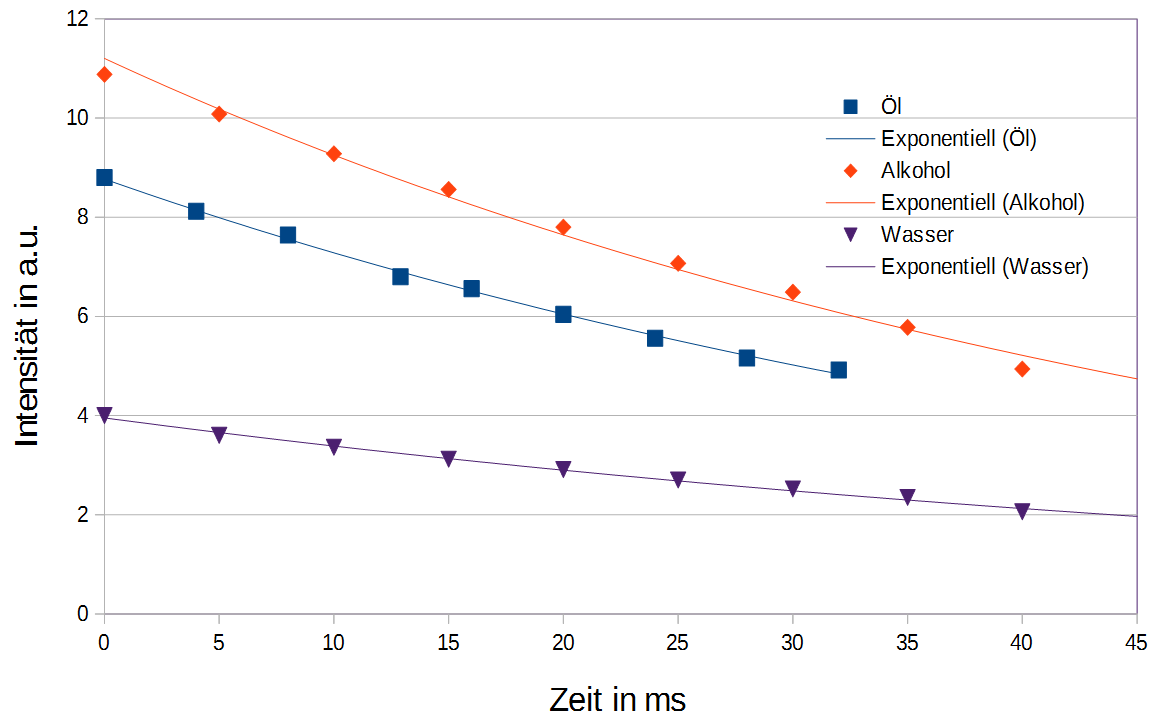
\includegraphics[width=1\textwidth]{pics/T1}
			\caption{Es sind die gemessenen Magnetisierung in der x-y-Ebene in arbiträren Einheiten über die Zeit zwischen einem $90^\circ$-Puls und einem $180^\circ$-Puls (IR-Methode) für verschiedene Medien abgebildet. Die durchgelegten Linien entsprechen exponentiellen Fitfunktionen.}
			\label{abb:T1}
		\end{figure}
		
			Die ermittelten Zeiten weichen hierbei stark von den geschätzten Werten aus Tab.\ref{tab:1Puls90} ab. Das lässt sich wahrscheinlich auf eine schlechte Schätzung der Zeiten zurückführen, da die geschätzten Zeiten nicht für den $\nicefrac{1}{e}$-ten Teil der Maximalamplitude, sondern für den ungefähren  Nullwert des betrachteten Signal, was nicht den Relaxationszeiten entspricht.
		
	\subsection{Bestimmung von $T_2$ mit Hilfe der Spin-Echo-Methode}
	
	\begin{table}[h]
		\centering
		\caption{Durch Spin-Echo-Methode gemessene Zeiten für $T_2$ für die verschiedenen Medien}
		\begin{tabular}{c c}
			Material & $T_2\,/\,\mathrm{ms}$  \\ \hline
			Wasser 	& $132,6$  \\
			Alkohol & $21,3$  \\
			Öl 		& $25,4$ 
		\end{tabular}
		\label{tab:1T2}
	\end{table}
	\begin{figure}[h]
		\centering
		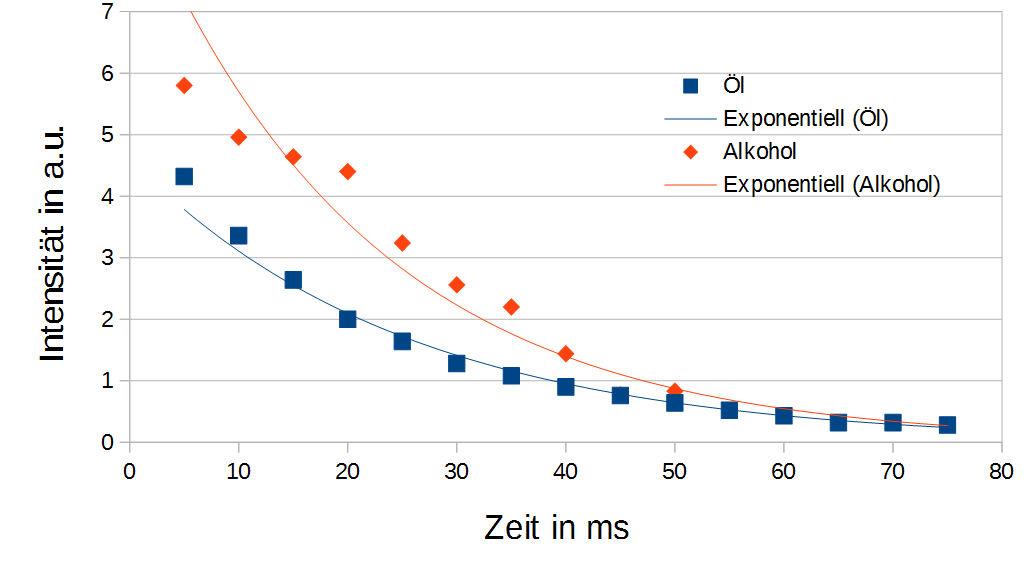
\includegraphics[width=1\textwidth]{pics/T2_1}
			\caption{Es sind die gemessenen Magnetisierung in der x-y-Ebene in arbiträren Einheiten über die Zeit zwischen einem $180^\circ$-Puls und einem $90^\circ$-Puls (Spin-Echo) für Öl und Alkohol. Die durchgelegten Linien entsprechen exponentiellen Fitfunktionen.}
			\label{abb:T2_1}
	\end{figure}
	\begin{figure}[h]
	\centering
	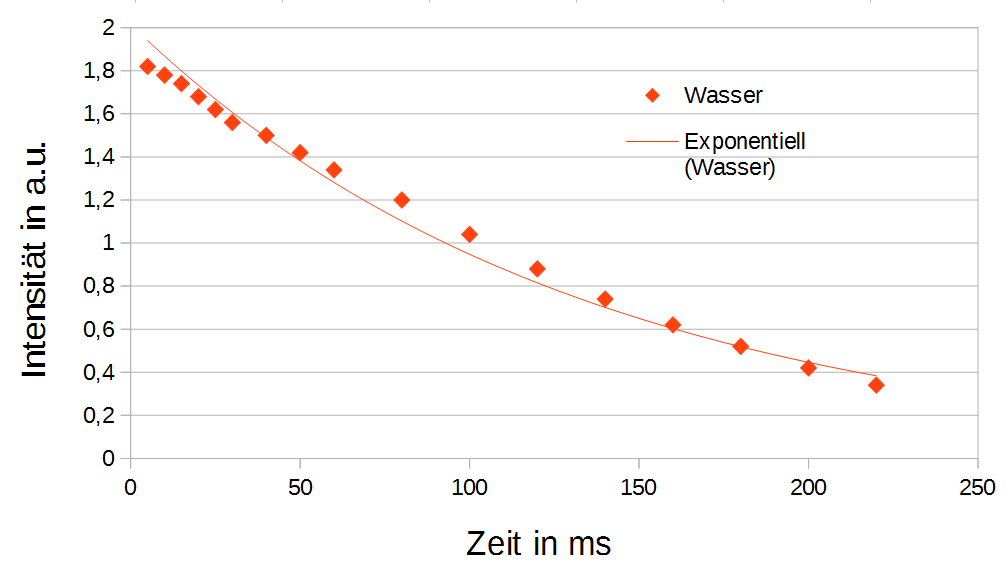
\includegraphics[width=1\textwidth]{pics/T2_2}
			\caption{Es sind die gemessenen Magnetisierung in der x-y-Ebene in arbiträren Einheiten über die Zeit zwischen einem $180^\circ$-Puls und einem $90^\circ$-Puls (Spin-Echo) für Wasser. Die durchgelegten Linien entsprechen exponentiellen Fitfunktionen.}
	\label{abb:T2_2}
	\end{figure}

	\section{Anhang}
	
		\bibliography{all.bib}
		\bibliographystyle{unsrt}

\end{document}